\section{Gaze control}
\label{Sec:gazecontrol}

One of the main modules in the reaching controller is represented 
by the {\tt gaze controller}. The control objective of this specific 
module consists in directing gaze toward a given target. The input of 
this module is represented by the target location in the image planes of 
the right and left eyes; this information is received by the {\tt target 
locator} module whose task is to find the target in the right and left 
image planes. The output instead consists in the head motor commands 
necessary to direct gaze toward the target. 

\begin{figure}[tbp]
\centering
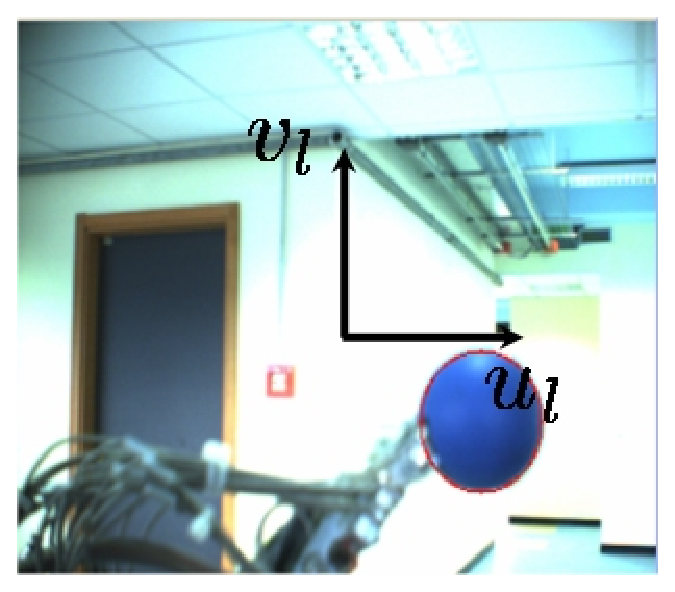
\includegraphics[width=25mm]{Figure/LeftImage.eps} \hspace{1cm}
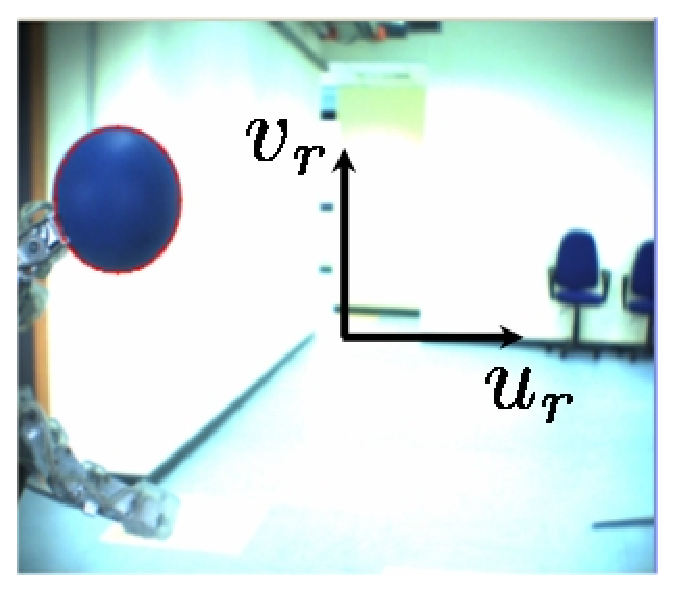
\includegraphics[width=25mm]{Figure/RightImage.eps}
\caption{Two typical images taken from the two cameras mounted on the 
eyes of the robot (resolution 320$\times$240). The ``attention system'' gives us the target position 
on the two image planes (in this case the center of the blue ball). 
The coordinates of the target on the right image plane will be denoted 
$u_r$, $v_r$, while on the left image will be denoted $u_l$, $v_l$. 
The {\tt gaze controller} task consists in moving the eyes and the 
neck in order to keep the target point at the center of the two image 
planes, i.e. $u_r = v_r = u_l = v_l = 0$.}
\label{Fig:ImagePlane}
\end{figure}
 
In this section we describe how this module has been implemented on James. 
The crucial aspect concerns the redundancy of the control problem as it 
has been stated above. In order to state this more clearly, we need to 
be more rigorous in defining the control task previously described as 
``directing gaze toward a given target''. Specifically, let $u_r$ and 
$v_r$ be the coordinates of the target on the right image plane. 
Similarly, let $u_l$ and $v_l$ be the coordinates of the target on the 
left image plane (see Figure \ref{Fig:ImagePlane}). The values of $u_r$, 
$v_r$, $u_l$, $v_l$ are the output of another module, the {\tt target 
locator}. Therefore, directing gaze toward the target consists in moving 
the neck and the eyes so as to obtain $u_r=0$, $v_r=0$, $u_l=0$, $v_l=0$. 
Let us define the vector 
$\tilde {\mathbf u}_{target}= \begin{bmatrix} u_r & v_r & u_l & v_l 
\end{bmatrix}^\top \in \mathbb R^4$ corresponding to the 
target location in the image planes. Assuming that the target is stationary 
with respect to the robot, we have that $\tilde {\mathbf u}_{target}$ 
can be expressed as a function of the head configuration 
$\mathbf q_{head} = \begin{bmatrix} \mathbf q_{eyes}^\top & \mathbf q_{neck}^\top \end{bmatrix}^\top \in \mathbb R^6$:
\begin{eqnarray*}
\tilde {\mathbf u}_{target} = \tilde f_{head} (\mathbf q_{head}),
\end{eqnarray*}
where the function $\tilde f_{head} : \mathbb R^6 \longrightarrow \mathbb R^4$ 
depeends on the head kinematics. Under suitable 
assumptions\footnote{The hypothesis is that we do not move the differential tilt, i.e. 
$\alpha_t^d = 0$ and that the camera optical axes are aligned 
with the pan rotation axes. See also Section \ref{sec:setup} 
for further details.}, we do not need to impose simultaneously 
the four conditions $u_r=0$, $v_r=0$, $u_l=0$, $v_l=0$ since one of them will be 
automatically satisfied given that the other three conditions are 
satisfied\footnote{In practice we have that if $u_l=0$, $v_l=0$ and $u_r=0$ then $v_r=0$. 
Alternatively, if $u_l=0$, $u_r=0$ and $v_r=0$ then $v_l=0$. This fact 
follows trivially considering that the target moves in a three dimensional 
space.}. Under this simplification we have that 
our control task can be redefined as the problem of controlling 
$\utarget = \begin{bmatrix} u_r & u_l & v_l \end{bmatrix}^\top \in \mathbb R^3$ 
to zero. The kinematic function will be in this case:
\begin{eqnarray*}
\utarget = f_{head} (\mathbf q_{head}), \qquad f_{head} : \mathbb R^6 \longrightarrow \mathbb R^3.
\end{eqnarray*}
Clearly, the task specification does not constrain all the head degrees of 
freedom. Roughly speaking\footnote{More formally, let $\bar {\mathbf q}_{head} = \begin{bmatrix} \bar 
{\mathbf q}_{eyes} & \bar {\mathbf q}_{neck} \end{bmatrix}$ 
be a fixating position, i.e. $f_{head}(\bar {\mathbf q}_{head}) = 0$. 
Moreover, let's assume that the given head configuration is non-singular, 
i.e. the Jacobian matrix: $$\frac{\partial f_{head}}{\partial \mathbf 
q_{head}}(\bar {\mathbf q}_{head}),$$ has full row rank. Then, by the 
implicit function theorem there exists a function 
$\mathbf q_{neck}(\cdot): \mathbb R^3 \longrightarrow \mathbb R^3$ 
(locally defined around $\bar {\mathbf q}_{eyes}$) such that 
$f_{head}({\mathbf q}_{eyes}, {\mathbf q}_{neck} ({\mathbf q}_{eyes}) ) = 0$ 
for all the configuration ${\mathbf q}_{eyes}$ belonging to the neighborhood 
of $\bar {\mathbf q}_{eyes}$.}, we are imposing 
$m=3$ constraints but we have $n=6$ free variables available so that we 
remain with $n-m=3$ additional degrees of freedom. Practically, we can have 
different configuration of the head ($\mathbf q_{head,1} \neq \mathbf 
q_{head,2}$) both keeping the same target in fixation 
(${\mathbf u}_{target,1} = {\mathbf u}_{target,2} = 0$). This 
redundancy issue has to be addressed carefully given the kinematic and 
dynamic properties of the head. Specifically, a trivial solution (such 
as constraining/blocking three degrees of freedom out of six) is not to be 
recommended since a good tracking behavior should involve all the  head 
degrees of freedom. In particular, a good tracker should take advantage of 
the eyes reduced inertia to perform fast movements; at the same time the 
eyes limited range of movements should be overcome by moving the neck which 
is instead capable of wider movements.

With these ideas in mind the strategy we have chosen consists in using the 
eyes version and common tilt to perform a sort of saccadic movement on the 
desired target and then to follow the movement of the eyes with the neck 
yaw and pitch, respectively. This choice is a consequence of the fact that 
the eyes can make fast movements because of their low inertia. However, 
their range of movement is small if compared to the neck which has a wider 
range even if with a larger inertia. This strategy allows us to keep the 
target at the center of the image while allowing fast and large movements 
of the target itself. Mathematically the above strategy can be implemented 
as follows:

\begin{eqnarray} \label{Eq:HeadEyeControl}
\left\{ \begin{matrix}
\dot {\alpha_v^c} &=&   K_p (u_l + u_r)\\
\dot {\theta_y} &=&   K_y \alpha_v^c \\
\dot {\alpha_t^c} &=&   K_t (v_l + v_r)\\
\dot {\theta_p} &=&   K_r \alpha_t^c
\end{matrix} \right.,
\end{eqnarray}
where $\alpha_t^c$ and $\alpha_v^c$ are the eyes version and common tilt and 
where $\theta_y$ and $\theta_p$ are the yaw and pitch movement of the neck. 
In the proposed control scheme, the vergence degree of freedom $\alpha_v^d$, 
which somehow corresponds to the distance of the target does not influence 
the neck position and is therefore controlled separately from the neck:
\begin{eqnarray} 
\dot {\alpha_v^d} &=&   K_p (u_l - u_r).
\end{eqnarray}
Finally, the neck roll degree of freedom $\theta_r$ is maintained fixed, 
i.e. $\theta_r^d=0$.

The proposed control strategy allows us to asymptotically fixate the target 
($u_l \rightarrow 0$, $v_l \rightarrow 0$, $u_r \rightarrow 0$ which 
implies $v_r \rightarrow 0$) while also also guaranteeing an asymptotically 
straight gaze ($\alpha_v^c \rightarrow 0$, $\alpha_t^c \rightarrow 0$). Moreover
, by choosing a suitable value for the gains $K_p$, $K_y$, $K_t$ and $K_r$ it
is possible to achieve an asymptotic behavior with the eyes moving rapidly on 
the target and the neck following the eye movement with a slower 
movement.
